\documentclass[10pt]{report}
\usepackage{/Users/bradenhoagland/latex/math}

\lhead{Braden Hoagland}
\chead{HW 8}
\rhead{}

\renewcommand{\theenumi}{\alph{enumi}}

\begin{document}
%\tableofcontents

\begin{exer}[]
\S 6.3 \#2.
\end{exer}
Suppose $k_1=0$ and $k_2$ is never 0, and suppose $\left\{ E_i \right\}$ is a principal frame field of $M$. If $\alpha$ is a principal curve of $k_1$, then by Theorem 1.4, $\alpha'' = \nabla_{E_1}E_1= \sum_{j=1}^{3} \omega_{ij}(E_1)E_j$. We know $\omega_{11}=0$, and since $\left\{ E_i \right\}$ is principal, $\omega_{13}(E_1)=k_1=0$. Also, by Theorem 2.6, $\omega_{12}(E_1)=E_2[k_1]/(k_1-k_2)$. But since $k_1=0$, this reduces to 0, so $\alpha''=0$. Thus $\alpha$ is a straight line.

\begin{exer}[]
\S 6.3 \#5.
\end{exer}
Suppose $k_1,k_2$ are constant on a surface $M$.
\begin{itemize}
	\item \textbf{Case 1:} $k_1=k_2$. If both are 0, then $M$ is part of a plane. If both are nonzero, then since $M$ must be everywhere umbilic, then by Theorem 3.3, $M$ is part of a sphere.
	\item \textbf{Case 2:} $k_1 \neq k_2$. Assume there is a principal frame field $\left\{ E_i \right\}$ on $M$. Since $k_1,k_2$ are constant, Theorem 2.6 says
		\begin{align*}
			E_1[k_2] &= (k_1-k_2)\omega_{12}(E_2)=0\\
			E_2[k_1] &= (k_1-k_2)\omega_{12}(E_1)=0.
		\end{align*} Since $k_1 \neq k_2$, the only way to have these expressions equal 0 is if $k_i=0$ or $\omega_{12}(E_i)=0$. Since $\omega_{12}(E_i)$ cannot be 0 for both $i=1,2$, this means that $k_i=0$ for one of the $i$. Without loss of generality, assume $k_1=0$ and $\omega_{12}(E_2)=0$. By the assumption that $k_1 \neq k_2$, $k_2$ can never be 0. Then by the previous exercise, the principal curves of $k_1$ are straight lines. They must also be parallel, as $\nabla_{E_2}E_1 = \omega_{12}(E_2)E_2 + \omega_{12}(E_2)E_3 = 0$. The principal curves in the $k_2$ direction have fixed nonzero curvature, so they are circles. Thus $M$ is part of a circular cylinder.
\end{itemize}
		We have gone through every case, showing that $M$ must be part of a sphere, a plane, or a circular cylinder.
		\pagebreak

\begin{exer}[]
\S 6.8 \#2.
\end{exer}
\begin{figure}[H]
	\centering
	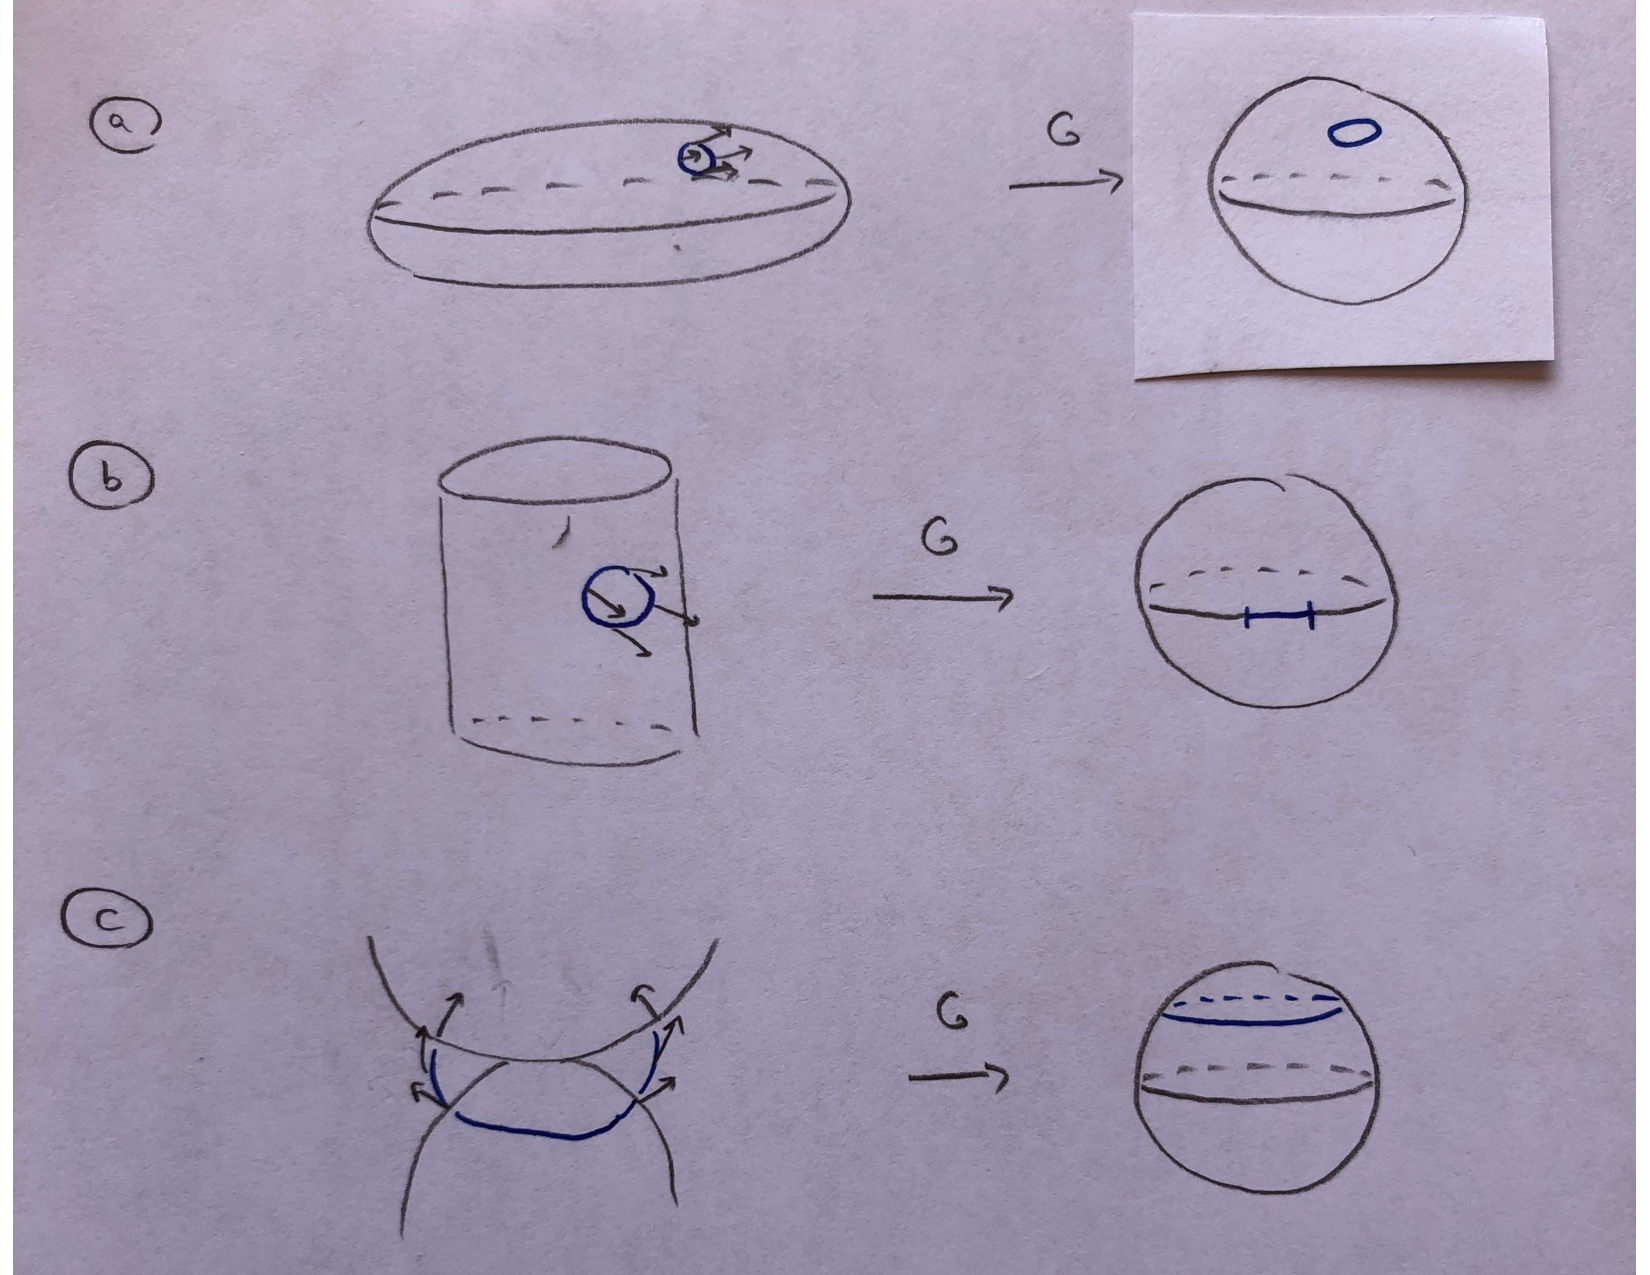
\includegraphics[scale=0.4]{fig/gauss.pdf}
	\caption{}
\end{figure}


\begin{exer}[]
\S 6.8 \#12.
\end{exer}
\begin{enumerate}
	\item By \S 5.4 \#2 (from HW 6), the Gaussian curvature of $S$ (before the Polar parameterization) is
		\[
			K = \frac{f_{uu}f_{vv}-f_{uv}^2}{(f_{u}^2+f_{v}^2+1)^2} = -\frac{1}{(u^2+v^2+1)^2} .
		\] Then after converting to polar coordinates it is
		\[
			K = -\frac{1}{(r^2+1)^2} .
		\] We can also parametrize $S$ with polar coordinates using the patch
		\[
			\mathbf{x}: (r,\theta) \mapsto  \left( r \cos\theta,r\sin\theta,r \right).
		\] We then calculate
		\[
		\mathbf{x}_{r}\times \mathbf{x}_{\theta} =
		\left|
		\begin{matrix}
			U_1 &U_2 & U_3 \\
			\cos\theta&\sin\theta&2r\cos\theta\sin\theta\\
			-r\sin\theta&r\cos\theta&r^2(\cos^2\theta-\sin^2\theta)
		\end{matrix}
		\right| = (-r^2\sin\theta,-r^2\cos\theta,r),
		\] 
		so the area form $dS$ is given by
		\[
			dS = {\Vert{\mathbf{x}_{r}\times \mathbf{x}_{\theta}}\Vert}dr\;d\theta = r(r^2+1)^{1/2}\;dr\;d\theta.
		\] We can now calculate the total curvature as
		\begin{align*}
			\int_{} \int_{S} K\;dS &= \int_{0}^{2\pi} \int_{0}^{\infty} (-r(r^2+1)^{-3/2})\;dr\;d\theta \\
					       &= \int_{0}^{2\pi} \left[ (r^2+1)^{-1/2} \right]_{r=0}^{r=\infty}\;d\theta \\
					       &= \int_{0}^{2\pi} (-1)\;d\theta \\
					       &= -2\pi.
		\end{align*}
	\item We can find a normal vector field by calculating the gradient of $xy-z$, which is
		\[
			\nabla_{}(xy-z) = \left( y,x,-1 \right).
		\] Converting to polar coordinates and normalizing gives unit normals
		\[
			\pm U = \pm \frac{1}{(r^2+1)^{1/2}} (r\sin\theta,r\cos\theta,-1).
		\] Over the range $0 < \theta \leq 2\pi$, the tuple $(\cos\theta,\sin\theta)$ never has repeated points, so $G(U)$ is one-to-one. Since $K$ is also clearly always negative, by Corollary 8.6 the total curvature is $\pm$ the area of $G(S)$. Since we can sweep out all the points that lie on and within the circle $S_1$ using our parameterization, and since the $z$-coordinate is always negative, this means $G(S)$ is the Southern hemisphere of $\Sigma$, which has area $2\pi$. This is the negative of our answer from part (a), so it agrees with the corollary.
\end{enumerate}

\begin{exer}[]
\S 7.1 \#2.
\end{exer}
Let $\left\langle \mathbf{v},\mathbf{w} \right\rangle=(\mathbf{v}\cdot \mathbf{w})/v^2(\mathbf{p})$ and $\alpha(t)=(r\cos t, r\sin t)$ for $0 < t < \pi$.
\begin{enumerate}
	\item The velocity of $\alpha$ is $\alpha'(t) = (-r \sin t, r\cos t)$, so its speed is
		\[
			{\Vert{\alpha'(t)}\Vert} = \sqrt{\left\langle \alpha'(t),\alpha'(t) \right\rangle} = \frac{\sqrt{\alpha'(t)\cdot \alpha'(t)} }{v(\alpha(t))} = \frac{1}{\cos t} = \csc t.
		\] 
	\item The length of $\alpha$ is
		\[
			\int_{0}^{\pi} {\Vert{\alpha'(t)}\Vert}\;dt = \int_{0}^{\pi} \csc t\;dt.
		\] But $\csc t \to \infty$ as $t \to 0,\pi$, so the Poincare length of $\alpha$ goes to $\infty$. The Euclidean length, on the other hand, is just half of the circle's circumference, i.e. $\pi r$.
	\item If we were working in the usual Euclidean plane, the area of this region would be
		\[
		\int_{0}^{\pi} \int_{0}^{r} \rho \;d\rho\;d\theta = \frac{1}{2} r^2 \pi,
	\] which is half the area of $S^1(r)$. If we're working in the Poincare half-plane, then the area form must be divided by $v^2(\mathbf{p})$. But as we approach the $u$-axis, $1/v \to \infty$, so the area under $\alpha$ is infinite in this case.
\end{enumerate}

\begin{exer}[]
\S 7.1 \#4.
\end{exer}
\begin{enumerate}
	\item The expression given is a formal sum of bilinear functions of $\mathbf{x}_{u}$ and $\mathbf{x}_{v}$, so it is as a whole bilinear. It is also symmetric because $\mathbb{R}$ commutes over multiplication. We now show that $\left\langle \mathbf{x}_{u},\mathbf{x}_{v} \right\rangle$ is positive definite.

		Suppose $ \mathbf{v}\neq 0$, then
		\begin{align*}
			\left\langle \mathbf{v},\mathbf{v} \right\rangle &= \alpha v_1^2+2bv_1v_2+v_2^2 \\
									 &= v_2^2\left( \alpha\left( \frac{v_1}{v_2}  \right)^2+2b\left( \frac{v_1}{v_2}  \right) +c\right).
		\end{align*}
		But since $b^2<ac$, we have $(2b)^2=4b^2 <4ac$, so the quadratic formula tells us that this quadratic polynomial has no roots, i.e. no nonzero $\mathbf{v}$ gives $\left\langle \mathbf{v},\mathbf{v} \right\rangle=0$.

		Now plugging in $\mathbf{v}=(1,0)$ gives $\left\langle \mathbf{v},\mathbf{v} \right\rangle=a^2>0$, where this last inequality follows from the assumption $a>0$. Since this polynomial is continuous, doesn't ever equal 0, and is positive at some other point, we know that it is always positive for nonzero $\mathbf{v}$. Then since $\left\langle 0,0 \right\rangle=0$, we have
		\[
		\left\langle \mathbf{v},\mathbf{v} \right\rangle\geq 0
		\] 
		and
		\[
		\left\langle \mathbf{v},\mathbf{v} \right\rangle=0 \iff \mathbf{v}=0.
		\] Thus this satisfies the properties of an inner product.

	\item We can use the definition of $\left\langle \;,\; \right\rangle$ from part (a). The uniqueness of $\left\langle \;,\; \right\rangle$ follows from extending linearly to all tangent vectors instead of just $\mathbf{x}_{u}, \mathbf{x}_{v}$.
\end{enumerate}
\pagebreak

\begin{exer}[]
\S 7.1 \#7.
\end{exer}
We will use the fact that
\begin{align*}
	F_{*}(U_1) &= f_{u}U_1+g_{u}U_2 \\
	F_{*}(U_2) &= f_{v}U_1 + g_{v}U_2.
\end{align*}

\textbf{Forward:} Suppose $F$ is conformal and orientation-preserving. Then
\begin{align*}
	f_{v}U_1+g_{v}U_2 &= F_{*}U_2 \\
			  &= F_{*}(JU_1).
			  \intertext{Since $F$ is conformal and orientation-preserving, $F_{*}$ commutes with $J$, so this becomes}
			  &= J(F_{*}U_1) \\
			  &= J(f_{u}U_1+g_{u}U_2) \\
			  &= f_{u}JU_1+g_{u}JU_2\\
			  &= f_{u}U_2-g_{u}U_1.
\end{align*}
This implies $f_{u}=g_{v}$ and $f_{v}=-g_{u}$.

\textbf{Backward:} Suppose $f_{u}=g_{v}$ and $f_{v}=-g_{u}$. Then
\[
	\left\langle F_{*}U_1,F_{*}U_2 \right\rangle = f_{u}f_{v}+g_{u}g_{v} = f_{u}f_{v}-f_{u}f_{v}=0
\] and
\[
\left\langle F_{*}U_1,F_{*}U_1 \right\rangle= f_{u}^2+g_{u}^2 = \left| \frac{dF}{dz}  \right|^2 = f_{v}^2+g_{v}^2 = \left\langle F_{*}U_2,F_{*}U_2 \right\rangle.
\] Thus $F$ is conformal with scale factor $|dF/dz|$. It's orientation preserving since
\[
J_{F} = f_{u}g_{v}-f_{v}g_{u} = f_{u}^2+f_{v}^2 > 0.
\] Note that the inequality is strict because $F$ is regular.

\end{document}
